%qqqqqqqqqqqqqqqqqqqqqqqqqqqqqqqqqqqqqqqqqqqqqqqqqqqqqqqqqqqqqqqqqqqqqqqqq
%Quote
\begin{savequote}[50mm]
‘‘The Cosmos is all that is or was or ever will be. Our feeblest contemplations 
of the Cosmos stir us: there is a tingling in the spine, a catch in the voice, 
a faint sensation, as if a distant memory, of falling from a height. We know 
we are approaching the greatest of mysteries.’’

\qauthor{Carl Sagan}
\end{savequote}
%qqqqqqqqqqqqqqqqqqqqqqqqqqqqqqqqqqqqqqqqqqqqqqqqqqqqqqqqqqqqqqqqqqqqqqqqq




%#########################################################################
\chapter{Theoretical Framework in Cosmology}
\label{cha:Theoretical Framework}


%Reviewed
The aim of this chapter is to cover, in a self-contained and summarized 
way, all the theoretical framework needed for the study of the large-scale
universe. From the simplest models of the universe given by Friedman's 
solutions, the theory of perturbations for the formation of complex 
structures like galaxies and galaxy clusters, until the schemes to 
quantify the cosmic web.



%#########################################################################




%*************************************************************************
%Isotropic and homogeneous universe
\section{Isotropic and Homogeneous Universe}
\label{sec:IsotropicAndHomogeneousUniverse}


%Reviewed
The two big pillars of the modern cosmology are the cosmological principle
and the theory of the general relativity. The first one is a principle 
where it is assumed that the universe is isotropic and homogeneous at very
large scales, while the second one gives the theoretical support needed in 
order to understand properly the relation between the matter content of 
the universe and the structure of the space-time.


%Reviewed
As it has been evidenced by observations of large-scale structures and the 
CMB, the universe appears to be isotropic and homogeneous at large scales,
which is in agreement with the cosmological principle. Moreover, this fact
simplifies quite enough the complex tensorial formulation of the general
relativity, thereby allowing finally leading to the Friedmann's equations.



	%---------------------------------------------------------------------
	%Curved space metric
	\subsection{Metric of Curved Spaces}
	\label{subsec:MetricOFCurvedSpaces}
	%---------------------------------------------------------------------

	
%Reviewed
In the construction of an isotropic and homogeneous model of universe, it 
is necessary to establish an adequate metric which describes it properly. 
An illustrative example that could be generalized is a 2D spherical 
surface, which clearly satisfies the criteria of homogeneity and isotropy.



%.........................................................................
%2D sphere
\begin{figure}[htbp]
	\centering
	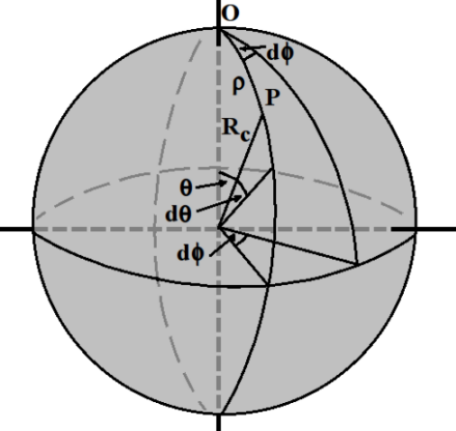
\includegraphics[width=0.5\textwidth]
	{./figures/2_theoretical_framework/2D_Sphere.png}
	
	\caption{\small{Metric of a spherical surface.}}
	
	\label{fig:2sphere}
\end{figure}
%.........................................................................


%Reviewed
A line element over the surface shown in the figure \ref{fig:2sphere} can
be described as


%Reviewed
%.........................................................................
%Line element on the sphere
\[ dl^2 = d\rho^2 + R_c^2 \sin^2 \pr{ \frac{\rho}{R_c}}d\phi^2 \]
%.........................................................................
where it have been introduced a new length coordinate over the surface, 
defined as $\rho = \theta R_c$ and $R_c$ is the curvature radius of the 
sphere. Another very convenient way to rewrite this expression, and that 
allowing a very useful generalization, it is reached defining the curvature
parameter $k$ and the coordinate $r = \sin (\rho/a)$, obtaining:


%Reviewed
%.........................................................................
%Line element on the sphere with time-dependent curvature
\[ dl^2 = a^2(t) \cor { \frac{dr^2}{1-kr^2} + r^2 d\phi^2 } \]
%.........................................................................
with $k = -1$ and it is assumed a time-dependent curvature radius $R_c = 
a(t)$. The metric in this case is 3D and is obtained by replacing the 
differential element of angle $d\phi^2$ by the solid angle differential 
$d\Omega^2 = d\theta^2 + \sin^2\theta d\phi^2$.


 
%.........................................................................
%Line element on the 3-sphere
\eq{eq:LineElement3D}
{ dl^2 = a^2(t) \cor { \frac{dr^2}{1-kr^2} + r^2 (d\theta^2 + 
\sin^2\theta d\phi^2)} }
%.........................................................................


%Reviewed
Finally, time is included, so the space-time interval for the metric of
isotropic and homogeneous curved spaces is:



%.........................................................................
%Interval element on the 3-sphere
\eq{eq:IntervalCurvedSpaces}
{ ds^2 = c^2 dt^2 - a^2(t) \cor { \frac{dr^2}{1-kr^2} + r^2 (d\theta^2 + 
\sin^2\theta d\phi^2)} }
%.........................................................................


%Reviewed
The direct generalization of this expression consists in varying the 
different values of the curvature parameter $k$ in order to obtain the 
metric of flat ($k = 0$), spherical closed ($k = -1$) or opened spaces
($k = 1$), as it is shown in \cite{longair2008} or \cite{padmanabhan1995}.


\
%.........................................................................
%Curved Spaces
\begin{figure}[htbp]
	\centering
	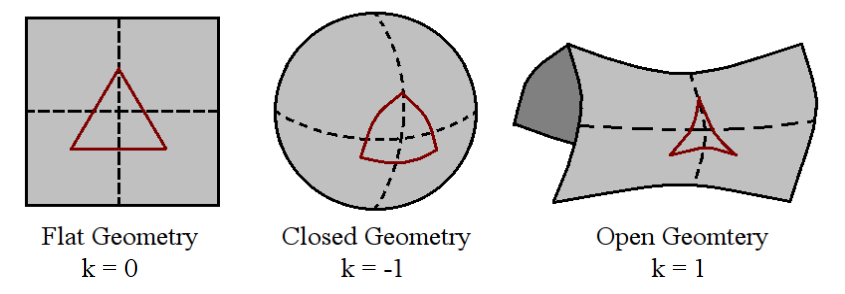
\includegraphics[width=0.9\textwidth]
	{./figures/2_theoretical_framework/Curved_Spaces.png}

	\caption{\small{Curved spaces according to the curvature parameter.}}
	
	\label{fig:CurvedSpaces}
\end{figure}
%.........................................................................
\

%Reviewed
An alternative way to rewrite the metric is introducing two changes of 
coordinates defined as



%.........................................................................
%Xi variable
\[ \chi = \int \frac{ dr'}{\sqrt{1 - k r'^2}}\]
%.........................................................................


%Reviewed
%.........................................................................
%Proper time
\[ \tau = \int \frac{ c dt'}{a(t')}\]
%.........................................................................
where each one is respectively interpreted as a length coordinate over the 
hypersurface that defines the space ($\chi$) and as the proper time 
measured locally ($\tau$). It is obtained the next expressions for the 
metric



%.........................................................................
%Interval element generalized
\eq{eq:IntervalCurvedSpacesAltern1}
{ ds^2 = c^2 dt^2 - a^2(t) \cor { d\xi^2 +  f^2_k(\xi)(d\theta^2 + 
\sin^2\theta d\phi^2)} }
%.........................................................................


%Reviewed
%.........................................................................
%Interval element generalized
\eq{eq:IntervalCurvedSpacesAltern2}
{ ds^2 = \bar a^2 (\tau)\cor{ d\tau^2 - d\xi^2 -  f^2_k(\xi)(d\theta^2 + 
\sin^2\theta d\phi^2)} }
%.........................................................................
where the function $f_k(\chi)$ is defined according to the value of the 
curvature parameter.



%.........................................................................
%Curvature Function
\eq{eq:CurvatureFunction}
{ f_k(\chi) = \left\{  \matrix{	
\sin \chi	&	k = 1		\cr 
\chi 		& 	k = 0 		\cr	
\sinh \chi 	& 	k = -1 		\cr } \right.  }
%.........................................................................


%Reviewed
In spite of the derived expressions for the metric 
\ref{eq:IntervalCurvedSpaces} \ref{eq:IntervalCurvedSpacesAltern1} and
\ref{eq:IntervalCurvedSpacesAltern2} are completely equivalent, the usage
of one or another depends on the specific problem. Especially the 
expression \ref{eq:IntervalCurvedSpacesAltern1} is usually more used and
is defined as the Friedmann's metric.


%Reviewed
It could be shown that in Riemannian manifolds \footnote{A Riemannian 
manifold is a space where it can be defined (well-defined) a metric.},
the space-time interval is expressed in terms of the metric tensor as
\cite{weinberg1972}


%Reviewed
%.........................................................................
%Metric-Interval relation
\[ ds^2 = g_{\mu \nu}dx^\mu dx_\nu \]
%.........................................................................
where it has been introduced the cuadrivector $x^\mu = 
(ct, r, \theta, \phi)$.


%Reviewed
Due to the assumption of isotropy and homogeneity, the metric tensor must
be diagonal, furthermore, comparing with the expression 
\ref{eq:IntervalCurvedSpaces}, it is possible to obtain the next explicit 
form



%.........................................................................
%MetricTensor
\eq{eq:MetricTensor}
{g_{\mu \nu} = \pr{ \matrix{ 
1		&				0			&		0			&				0				\cr
0		&	-a^2(t)(1 - kr^2)^{-1}	&	 	0			&				0				\cr
0		&				0			&	-a^2(t)r^2		&				0				\cr
0		&				0			&		0			&	-a^2(t)r^2 \sin^2 \theta } }}
%.........................................................................


%Reviewed
From this metric and the Einstein's field equations, it is possible to 
build simple models of the universe, such as it shall be shown in the 
subsection \ref{subsec:GeneralRelativityAndFriedmannEquations}.



			%-------------------------------------------------------------
			%Measuring distances
			\subsubsection*{Measuring distances}
			%-------------------------------------------------------------


%Reviewed
Once defined the metric of curved spaces, it is very useful to introduce
some concepts related with distances, which are used recurrently 
\cite{longair2008}. For the sake of simplicity it will be assumed a flat 
metric ($k = 0$).


%Reviewed
\begin{itemize}
%Comovil Radial Distance..................................................
\item \textit{\textbf{Comovil radial distance:}} by definition, a light
signal has an associated null interval, i.e. $ds^2 = 0$. Using the 
expression \ref{eq:IntervalCurvedSpaces} for the metric, it is obtained


%Reviewed
%.........................................................................
%Comovil Distance
\eq{eq:ComovilDistance}
{ r = \int_t^{t_0} \frac{ cdt'}{a(t')} = \int_a ^1 \frac{ c da}{a \dot a} }
%.........................................................................
where the specific form of $a(t)$ depends on the specific chosen cosmology
(see subsection \ref{subsec:SimpleSolutionsOfTheUniverse}) and $t_0$ is the
reference time, which is taken as the current age of the universe.


%Reviewed
Due to the assumption of an expanding metric, the distance between two 
objects depends on the time in which the measurement is performed. 
Moreover, the distance cannot be determined from a beam of light since
light has a finite velocity \footnote{$c=299\ 792\ 458$ m/s}. Because of 
that, it must be performed a projection on the light-cone traced by the 
beam in the current time, such as it is made in the expression 
\ref{eq:ComovilDistance}. The latter allows interpreting $r$ as the 
distance to an object in the current time, and it is quite different to
the apparent distance which corresponds to the time when the object in 
question emitted the observed light.


%Reviewed
%Proper Radial Distance..................................................
\item \textit{\textbf{Proper radial distance:}} by virtue of the 
definition of scale factor, to obtain the distance to an object in any 
time, it is enough to multiply the comovil distance by the scale factor 
evaluated in the same time, that is



%.........................................................................
%Proper Distance
\eq{eq:ComovilDistance}
{ r_{\submath{prop}} = a(t)\int_t^{t_0} \frac{ cdt'}{a(t')} = 
a\int_a ^1 \frac{ c da}{a \dot a} }
%.........................................................................	


%Reviewed
%Particle Horizon........................................................
\item \textit{\textbf{Particle horizon:}} considering a beam travelling 
through vacuum since the beginning of all time, at $t=0$; the maxim proper
distance that could be travelled by the light in a time $t$ is denominated 
particle horizon and determines all regions in the universe that could 
have been causally connected in that time. 



%.........................................................................
%Particle Horizon distance
\eq{eq:HorizonDistance}
{ r_{\submath{H}} = a(t)\int_0^{t} \frac{ cdt'}{a(t')} = 
a\int_0 ^a \frac{ c da}{a \dot a} }
%.........................................................................

\end{itemize}
	%---------------------------------------------------------------------
	%General relativity and Friedmann equations
	\subsection{General Relativity and Friedmann's Equations}
	\label{subsec:GeneralRelativityAndFriedmannEquations}
	%---------------------------------------------------------------------
	

%Reviewed
The Einstein's field equations of the general relativity play a fundamental
role since they express explicitly the relation between the matter 
content of the universe and the local geometry of the space-time.


%Reviewed
%.........................................................................
%EinsteinEquations
\eq{eq:EinsteinEquations}
{ R_{\mu \nu} - \frac{1}{2}R - g_{\mu \nu}\Lambda = 
\frac{8\pi G}{c^4}T_{\mu \nu} }
%.........................................................................
or equivalently


%Reviewed
%.........................................................................
%Einstein Equations Alternative
\eq{eq:EinsteinEquationsAltern}
{ R_{\mu \nu} + g_{\mu \nu}\Lambda = 
\frac{8\pi G}{c^4}\pr{T_{\mu \nu} - \frac{1}{2}T g_{\mu \nu}} }
%.........................................................................
where $T$ is the trace of the energy-momentum tensor (see 
\ref{eq:MomentumEnergyTensor}), $R_{\mu \nu}$ the Ricci curvature tensor
and $R$ the scalar curvature. The last two terms are calculated from 
different traces of the Riemann curvature tensor, as $R_{\mu \nu} = 
R^\eta_{\ \mu \eta \nu}$ and $R = R^{\mu}_{\ \mu}$. For convenience, it
has been introduced the term associated with the cosmological constant, 
which will be used below to calculate different models of the universe 
with dark energy contribution.


%Reviewed
The Riemann curvature tensor quantifies deviations of the metric of curved 
space-times with respect to the Euclidean metric and allows to determinate
completely the geometrical properties like the local curvature, different 
measures of distances and angles, etc. \cite{weinberg1972}. This tensor is
built from the Levi-Civita connection as


%Reviewed
%.........................................................................
%Riemann Tensor
\eq{eq:RiemannTensor}
{ R^\mu_{\ \nu \alpha \beta} = 
\Gamma^\mu_{\ \nu \alpha, \beta} -  
\Gamma^\mu_{\ \nu \beta, \alpha} + 
\Gamma^\mu_{\ \sigma \alpha}\Gamma^\sigma_{\ \nu \beta}-
\Gamma^\mu_{\ \sigma \beta}\Gamma^\alpha_{\ \nu \alpha}}
%.........................................................................
with the Levi-Civita connection defined from the metric as



%.........................................................................
%Afin Connection
\eq{eq:AfinConnection}
{ \Gamma^\nu _{\ \alpha \beta}  = \frac{1}{2}g^{\mu \sigma}
\pr{ g_{\sigma \alpha, \beta} + g_{\sigma \beta, \alpha} -
g_{\alpha \beta, \sigma} } }
%.........................................................................


%Reviewed
The right-hand side of the equation \ref{eq:EinsteinEquations} contains
the energy-momentum tensor $T_{\mu \nu}$, which characterizes the density
and the matter-energy flux of the universe. By virtue of the cosmological 
principle, this tensor must also be diagonal and if, furthermore, it is 
assumed an ideal fluid model, the next form is obtained



%.........................................................................
%MomentumEnergyTensor
\eq{eq:MomentumEnergyTensor}
{T^\mu_{\ \nu} = \pr{ \matrix{ 
c\rho^2	&	0	&	0	&	0				\cr
0		&	-P	&	0	&	0				\cr
0		&	0	&	-P	&	0				\cr
0		&	0	&	0	&	-P } }}
%.........................................................................


%Reviewed
Finally, using the equations \ref{eq:MetricTensor}, 
\ref{eq:EinsteinEquationsAltern} and \ref{eq:MomentumEnergyTensor}, it is 
possible to reduce the complex system of tensorial equations to two scalar
coupled equations which are usually called Friedmann's equations 
\cite{longair2008}. These equations describe completely the evolution of
an isotropic and homogeneous universe in terms of the scale factor $a(t)$ 
(see equation \ref{eq:LineElement3D})



%.........................................................................
%Friedmann Equation 1
\eq{eq:FriedmannEquation1}
{ \frac{\ddot a}{a} = -\frac{4\pi G}{3}\pr{\rho + \frac{3P}{c^2}}
+ \frac{c^2 \Lambda}{3}}
%.........................................................................


%.........................................................................
%Friedmann Equation 2
\eq{eq:FriedmannEquation2}
{ \frac{\ddot a}{a} + 2\frac{\dot a^2}{a^2} + 2\frac{c^2 k}{a^2} =
4\pi G \pr{ \rho - \frac{P}{c^2} } + c^2 \Lambda}
%.........................................................................


%Reviewed
In order to solve this equation system in terms of $a(t)$ and thereby 
obtaining the evolution of the scale factor, it is necessary to know the 
explicit time-dependent expression of the density $\rho$ and the pressure
$P$, or equivalently, the dependence on the scale factor. This must be done
for each type of energy-matter of the universe. A detailed derivation of
these explicit expressions could be found in \cite{longair2008} and they
are summarized in the table \ref{tab:PropertiesDependence}.



%.........................................................................
%Table of dependences of Matter-Energy content of the universe with a
\begin{table}[htbp]
\centering
\begin{tabular}{|c|c|c|c|} \hline
\cellc{\textbf{Property}} 	& 
\cellc{\textbf{Density}} 	&
\cellc{ \textbf{Pressure}}	& 
\cellc{\textbf{Temperature}}		\\ \hline

& & &  \\
\textbf{Matter}& $\rho = \rho_0 a^{-3}(t)$ & $p = p_0 a^{-5}(t)$ & $T = T_0 a^{-2}(t)$ \\ 
\small{(baryonic + dark)} & & &  \\ \hline
& & &  \\
\textbf{Radiation }& $\rho = \rho_0 a^{-4}(t)$ & $p = p_0 a^{-4}(t)$ & $T = T_0 a^{-1}(t)$ \\ 
\small{(+ relativistic matter)} & & &  \\ \hline
& & &  \\
\textbf{Vacuum }& $\rho = \rho_0 $ & $p = p_0 $ & $-$ \\ 
& & &  \\ \hline
\end{tabular}
\caption{Dependence of some quantities on the scale factor $a(t)$
\cite{longair2008}.}
\label{tab:PropertiesDependence}
\end{table}
%.........................................................................


%Reviewed
By convention, it has been taken the current scale factor as $a_0 = a(t_0) 
= 1$ and the reference values are defined as $\rho_0 = \rho(a_0)$, $P_0 = 
P(a_0)$ and $T_0 = T(a_0)$. Using the Friedmann's equations, defining the
Hubble parameter as $H(t) = \dot a/ a$ and the vacuum density as 
$\rho_\Lambda = c^2\Lambda/8\pi G$, it is obtained



%.........................................................................
%Pre Hubble Equation
\[ \pr{ \frac{\dot a}{a} }^2 = H^2(t) = \frac{ 8\pi G}{3}
\cor{ \rho_{m}\frac{1}{a^{3}} + \rho_{r}\frac{1}{a^{4}} + \rho_{\Lambda} }
- \frac{ c^2 k }{a^2} \]
%.........................................................................


%Reviewed
Evaluating this expression in the current epoch $H(t_0) = H_0$, with $H_0$
the Hubble constant and defining the critical density $\rho_c$ as the 
density that the universe must have in order to be flat.


%Reviewed
%.........................................................................
%Critical Density
\eq{eq:CriticalDensity}
{ \rho_c = \frac{3H_0^2}{8\pi G} }
%.........................................................................
it leads to the equation of evolution for the Hubble parameter


%Reviewed
%.........................................................................
%Hubble Equation
\eq{eq:HubbleEquation}
{ H^2(t) = H_0^2 \cor{ 
(1 - \Omega_0)\frac{1}{a^2} +  
\Omega_m \frac{1}{a^3} +
\Omega_r \frac{1}{a^4} +
\Omega_\Lambda} }
%.........................................................................
where it has been introduced the density parameters $\Omega_i$, defined
as the current density of the i-th specie in the current epoch, normalized 
with the critical density \ref{eq:CriticalDensity}, and $\Omega_0 = 
\sum_i \Omega_i$. These density parameters along with the Hubble constant
are part of the free parameters of the theory and must be determined by 
observations. This allows to characterize different particular cosmologies
\footnote{\textit{Cosmology} must be understood in this context as a 
specific solution of the Friedmann's equations.}



	%---------------------------------------------------------------------
	%Simple solutions of the universe
	\subsection{Simple Solutions of the Universe}
	\label{subsec:SimpleSolutionsOfTheUniverse}
	%---------------------------------------------------------------------


%Reviewed
Although in this stage it has not been introduced the complete formalism 
of small perturbations and structure formation, the set of equations
\ref{eq:FriedmannEquation1}, \ref{eq:FriedmannEquation2} and 
\ref{eq:HubbleEquation} leads to a first and rough understanding of the
evolution of the Universe.


%Reviewed
In this subsection will be presented some analytic solutions to the 
Friedmann's equations. In spite of the ideal assumptions on which are
based, in some cases, they can be used as approximations in some stages
of evolution of the universe, thus allowing a physical understanding more 
adequate than exact numerical solutions.



			%-------------------------------------------------------------
			%Einstein-de Sitter Universe
			\subsubsection*{Einstein - de Sitter Universe}
			%-------------------------------------------------------------


%Reviewed
The Einstein-de Sitter Universe is a cosmological model with a flat metric
and composed entirely of matter, this implies that $\Omega_0 = \Omega_m = 1$ 
and $k=0$. Applying this in equation \ref{eq:HubbleEquation}, it is obtained
the next expression



%.........................................................................
%EinsteindeSitter
\eq{eq:EinsteindeSitter}
{ H^2(t) = \pr{\frac{\dot a}{a}}^2 = H_0^2 \frac{1}{a^3} }
%.........................................................................


%Reviewed
Integrating, it leads to the explicit time-dependent solution for the 
scale factor



%.........................................................................
%EinsteindeSitterSolution
\eq{eq:EinsteindeSitterSolution}
{ t(a) = \frac{ 2}{3H_0} a ^{3/2} }
%.........................................................................


%Reviewed
Although in this case it is possible to obtain the explicit form of $a(t)$,
most of the time it is only possible to have the implicit solution $t(a)$.
Another very useful way to describe this solution is by using the redshift
$z$, which is related with the scale factor as \cite{longair2008}


%Reviewed
%.........................................................................
%Redshift
\eq{eq:Redshift}
{ z + 1 = \frac{ a_0}{a} }
%.........................................................................
to finally obtain



%.........................................................................
%EinsteindeSitterSolutionZ
\eq{eq:EinsteindeSitterSolutionZ}
{ t(a) = \frac{ 2}{3H_0} (1+z) ^{-3/2} }
%.........................................................................


%Reviewed
This solution is quite close to the real behaviour of the universe in the 
matter-dominated epoch, between $70000$ and $5$ millions of years after 
the Big Bang \cite{padmanabhan1995}.



			%-------------------------------------------------------------
			%Radiation Dominated Universe
			\subsubsection*{Radiation-Dominated Universe}
			%-------------------------------------------------------------


%Reviewed
In this case, it will be assumed that the universe is radiation-dominated, 
that is $\Omega_0 = \Omega_r$, but not necessarily flat. The Friedmann's 
equations lead to the next expression



%.........................................................................
%Radiation Universe
\eq{eq:RadiationUniverse}
{ H^2(t) = \pr{\frac{\dot a}{a}}^2 = H_0^2 \cor{ 
(1 - \Omega_r)\frac{1}{a^2} +  \Omega_r \frac{1}{a^4}} }
%.........................................................................


%Reviewed
Integrating this expression, it is obtained the next implicit solution for
the scale factor


%Reviewed
%.........................................................................
%Radiation Universe Solution
\eq{eq:RadiationUniverseSolution}
{ t = \left\{  \matrix{ 
H_0^{-1}(\Omega_r - 1)^{-1}\pr{ \Omega_r^{1/2} - 
\cor{a^2(1-\Omega_r) + \Omega_r}^{1/2} } & \Omega_r \neq 1 \cr
H_0^{-1} a^2/2 & \Omega_r = 1} \right. }
%.........................................................................
or in terms of redshift



%.........................................................................
%Radiation Universe Solution Z
\eq{eq:RadiationUniverseSolutionZ}
{ t = \left\{  \matrix{ 
H_0^{-1}(\Omega_r - 1)^{-1}\pr{ \Omega_r^{1/2} - 
\cor{(1+z)^{-2}(1-\Omega_r) + \Omega_r}^{1/2} } & \Omega_r \neq 1 \cr
H_0^{-1} (1+z)^{-2}/2 & \Omega_r = 1} \right. }
%.........................................................................


%Reviewed
This solution is useful as an approximation for the radiation-dominated 
epoch, which happened from the big bang until the recombination epoch, 
approximately $380 000$ years after the big bang, or equivalently in a
redshift of $z = 1100$ \cite{padmanabhan1995}.



			%-------------------------------------------------------------
			%Vacuum Dominated Universe
			\subsubsection*{Vacuum-dominated Universe}
			%-------------------------------------------------------------
		

%Reviewed	
This type of hypothetical universe is completely vacuum-dominated, or
equivalently dominated by the cosmological constant. Making $\Omega_0 = 
\Omega_\Lambda$ in the Friedmann's equations, it is obtained
			


%.........................................................................
%Vacuum Universe
\eq{eq:VacuumUniverse}
{ H^2(t) = \pr{\frac{\dot a}{a}}^2 = H_0^2 \cor{ 
(1 - \Omega_\Lambda)\frac{1}{a^2} +  \Omega_\Lambda} }
%.........................................................................


%Reviewed	
Solving for $t(a)$


%Reviewed
%.........................................................................
%Vacuum Universe Solution
\eq{eq:VacuumUniverseSolution}
{ t = \frac{1}{H_0^2 \Omega_\Lambda^{1/2}}
\ln\cor{ a \pr{ \frac{\Omega_\Lambda}{1 - \Omega_\Lambda} }^{1/2} +
\pr{ 1 + \frac{\Omega_\Lambda}{1 - \Omega_\Lambda}a^2 }^{1/2} } }
%.........................................................................
and using the redshift



%.........................................................................
%Vacuum Universe Solution Z
\eq{eq:VacuumUniverseSolutionZ}
{ t = \frac{1}{H_0^2 \Omega_\Lambda^{1/2}}
\ln\cor{ \frac{1}{1+z} \pr{ \frac{\Omega_\Lambda}{1 - \Omega_\Lambda} }^{1/2} +
\pr{ 1 + \frac{\Omega_\Lambda}{1 - \Omega_\Lambda}\frac{1}{\pr{1+z}}^2 }^{1/2} } }
%.........................................................................


%Reviewed
This solution is very interesting because, unlike the previous solutions, 
is only valid for values of the density parameter within the range 
$0<\Omega_\Lambda <1$. This implies that it is not possible to have a  
universe with flat or hyperbolic geometry when it is vacuum-dominated.
Another aspect equally remarkable is the concavity of the scale factor 
$a(t)$ obtained from \ref{eq:VacuumUniverseSolution} (see figure 
\ref{fig:Cosmologies}), which shows an accelerated expansion of the 
universe. This characteristic is only possible when there is a non-null 
term associated to the vacuum energy.


%Reviewed
Finally and like the previous solutions, the expression 
\ref{eq:VacuumUniverseSolution} can be used as an approximation for the
vacuum-dominated epoch of the universe, which lasts from the end of the
matter-dominated epoch, $5$ millions of years after the big bang, until 
nowadays \cite{longair2008}.



			%-------------------------------------------------------------
			%WMAP7 Universe
			\subsubsection*{WMAP7 Universe}
			%-------------------------------------------------------------
			
			
%Reviewed
The set of parameters associated to the standard cosmological model has 
been measured on several occasions by different spacecraft missions (see
section \ref{sec:CosmologicalObservations}). Among those measurements it 
is notable the one conducted by WMAP. The data obtained after seven years
of observation (WMAP7) are adopted in this work \cite{WMAP7}. Among the 
cosmological parameters measured are the Hubble constant and the density
parameters $\Omega_i$. Taking the values given in the table 
\ref{tab:CosmologicalParameters} and for simplicity assuming $\Omega_0 = 1$
it is possible to integrate the Friedmann's equations

			
%Reviewed	
%.........................................................................
%WMAP Universe
\eq{eq:WMAPUniverse}
{ H^2(t) = H_0^2 \cor{ 
\Omega_m \frac{1}{a^3} +
\Omega_r \frac{1}{a^4} +
\Omega_\Lambda} }
%.........................................................................
to obtain


%.........................................................................
%WMAP Universe
\eq{eq:WMAPUniverse}
{ t = \frac{1}{H_0}\int _0 ^{a}\cor{ 
\Omega_m \frac{1}{a'} + 
\Omega_r \frac{1}{a'^2} +
\Omega_\Lambda a'^2 }^{-1/2}da' }
%.........................................................................

\
%.........................................................................
%Friedmann Solutions
\begin{figure}[htbp]
	\centering
	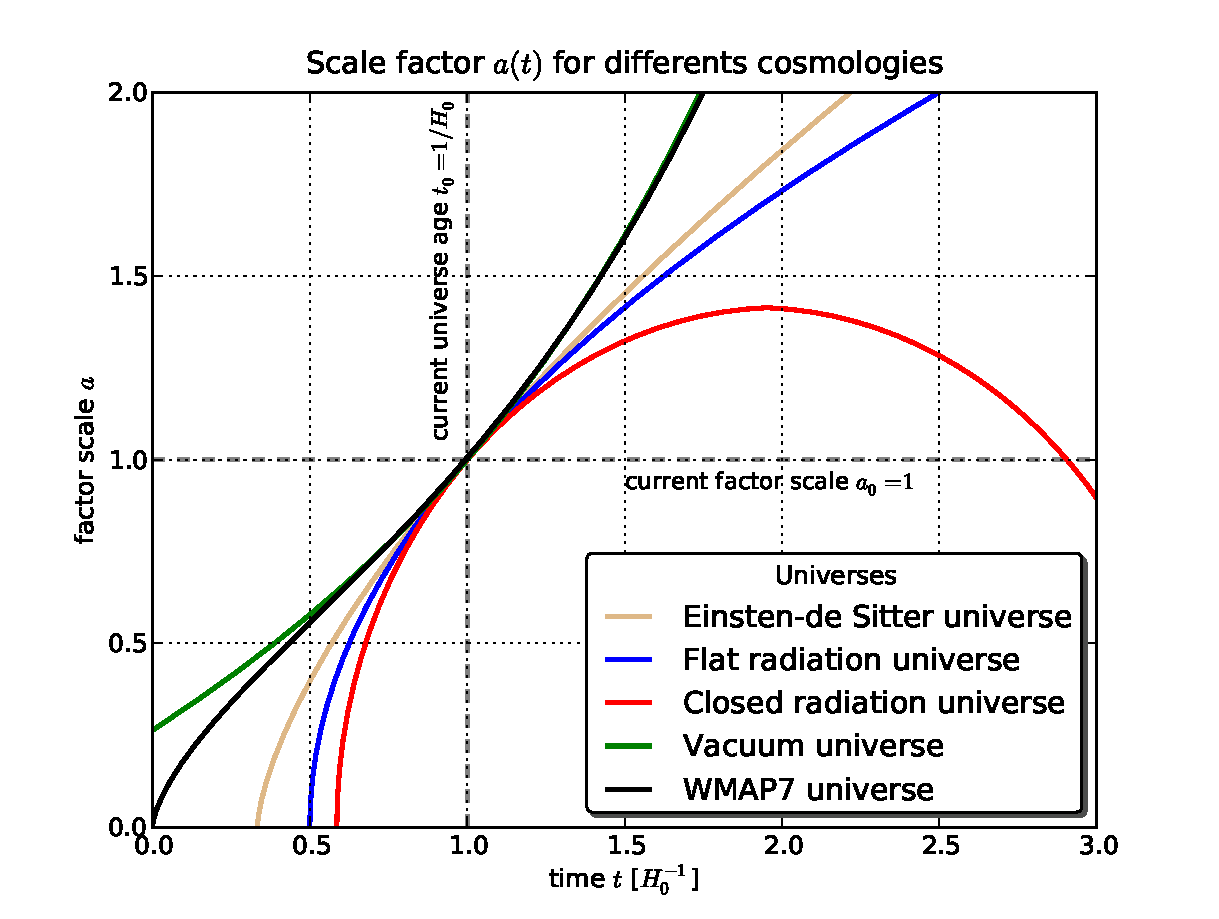
\includegraphics[width=0.9\textwidth]
	{./figures/2_theoretical_framework/Friedmann_Solution.pdf}

	\caption{\small{Different solutions of the universe according to the
	Friedmann's equations.}}
	
	\label{fig:Cosmologies}
\end{figure}
%.........................................................................
\

%Reviewed
It is possible to obtain an analytic solution of this integral in terms of
elliptic functions, but for simplicity it is chosen the numerical solution.
In the figure \ref{fig:Cosmologies} is shown the solution for a WMAP7 
universe and it is compared with other cosmologies, derived previously.


%Reviewed
An interesting characteristic of the solution for the WMAP7 universe is 
the change of concavity (black curve in the figure \ref{fig:Cosmologies}), 
which indicates a transition from the matter/radiation-dominated epoch
to an accelerated expanding regime associated to the vacuum energy.
Another important aspect is the prediction of the age of the universe.
Taking into account the previously defined normalization for the scale
factor $a(t_0) = a_0$, it is straightforward to see that $t_0 = H_0^{-1} 
\approx 13.75 \times 10^9$ years. Other cosmologies under the same 
normalization predict different ages, since larger values such as a 
vacuum-dominated universe, until smaller and even a collapse time (usually
known as big crunch time) such as a radiation-dominated and closed 
universe.



%*************************************************************************




%*************************************************************************
%Linear Structure Formation
\section{Linear Regime of Structure Formation}
\label{sec:LinearStructureFormation}


%Reviewed
The previous section deals about the universe as a whole, assuming as 
valid the condition of isotropy and homogeneity. Although the real universe
has this asymptotic behaviour at very large scales, at smaller local scales
the behaviour is quite different, being even completely anisotropic and 
highly non-homogeneous. Life is certainly the most illustrative example of 
that, one of the highest non-linearities of the universe, and thus, 
planets, stars, galaxies, galaxy clusters, in the same decreasing order of 
inhomogeneity and anisotropy.


%Reviewed
The standard way to introduce these local structures in the universe is by
assuming as valid the solutions of the Friedmann's equations at very large 
scales, but considering inhomogeneities as perturbations of the model. 
First, in the linear regime, where the perturbations in the density field
are much smaller than the background mean density ($\delta \rho \ll 
\rho_b$), and after, in the non-linear regime, where the perturbations are
comparable or even larger ($\delta \rho \sim \rho_b$) (see section 
\ref{sec:NonLinearStructureFormation}).

 

	%---------------------------------------------------------------------
	%Newtonian Approximation
	\subsection{Newtonian Approximation}
	\label{subsec:Newtonian Approximation}
	%---------------------------------------------------------------------


%Reviewed
The frame of linear evolution can be presented in two ways. The first 
one is by considering a perturbative term in the energy-momentum tensor
$ \delta T_{\mu \nu}$ and linearizing the Einstein's field equations 
\ref{eq:EinsteinEquations} and finally solving for $\delta R_{\mu \nu}$



%.........................................................................
%Perturbative Einstein Equations
\eq{eq:PerturbativeEinsteinEquations}
{ \mathcal{L}( R_{\mu \nu}, \delta R_{\mu \nu} ) = 
\frac{8\pi G}{c^2}\pr{ T_{\mu \nu} + \delta T_{\mu \nu} } }
%.........................................................................


%Reviewed
Although this method is, rigorously, more adequate, it has an inconvenience
which makes it very complicated of applying. Non-perturbative terms are 
not necessarily small in all the coordinate systems, inclusively, they can 
reach values with the same order or even bigger than the background mean 
density \cite{padmanabhan1995}.


%Reviewed
The second method consists in assuming perturbations with a comovil size
smaller than the Hubble radius ($r_\delta \ll r_H \sim cH_0^{-1}$)
\footnote{The Hubble radius $r_H$ is a length unit that defines the 
order of magnitude of the size of the observable universe.}, thereby
being possible to neglect relativistic effects due to the curvature
of the space-time. Once this is done, it is possible to use a Newtonian
scheme to evolve perturbations of the background universe. This scheme
assumes that the matter content of the universe is a fluid described by
three basic equations of fluid mechanics. The first one is the continuity
equation, which expresses mass conservation in a fluid



%.........................................................................
%Continuity equation
\eq{eq:ContinuityEquation}
{ \dtot{\rho}{t} = - \rho \nabla \cdot \bds u }
%.........................................................................


%Reviewed
The second one, Euler's equation, characterizes the velocity field of the 
fluid, and physically it expresses the momentum conservation law


%.........................................................................
%Euler Equation
\eq{eq:EulerEquation}
{ \dtot{\bds u}{t} = -\frac{ \nabla P}{\rho} - \nabla \varphi }
%.........................................................................


%Reviewed
And finally the Poisson's equation, which is the non-relativistic version
of the Einstein's field equations and expresses the relation between the
matter content of the universe and sources of gravitational field.

	
	
%.........................................................................	
%Poisson Equation
\eq{eq:PoissonEquation}
{ \nabla^2 \varphi = 4\pi G \rho }
%.........................................................................	


%Reviewed
In order to complete the Newtonian frame of perturbations is necessary to 
include in the previous system of equations (\ref{eq:ContinuityEquation}, 
\ref{eq:EulerEquation} and \ref{eq:PoissonEquation}) the effect of the 
expansion of the universe by making a change of coordinates of the proper
distance $\bds x$ to comovil distance $\bds r$


%Reviewed
%.........................................................................	
%Changing Coordinate
\[\bds x = a \bds r\]
%.........................................................................	
this implies that



%.........................................................................	
%Changing Coordinate
\[\bds u = \dtot{\bds x}{t} = 
\frac{\dot a}{a}\bds x + \bds v = \dot a \bds r + \bds v\]
%.........................................................................	


%Reviewed
This way to rewrite $\bds u$ allows separating the contribution of the 
expansion of the universe ($\dot a/a \bds x$), also called Hubble's law,
from the component due to the movement of the fluid, called peculiar 
velocity field and it is defined as $\bds v = a \dot{ \bds r}$.


%Reviewed
For the sake of simplicity it is decomposed the density field of the fluid 
into two parts, the background contribution and a perturbative term, that 
is $\rho = \bar \rho + \delta\rho = \bar \rho( 1+ \delta )$, where $\delta$
is called the density parameter and is dimensionless. In the case of the 
gravitational potential $\varphi$, it is defined a new field given by 
$ \Phi = \phi + \ddot a a r^2/2$ \cite{longair2008}. With these 
considerations it is finally obtained the final set of equations for 
describing a fluid in the Newtonian frame.


%Reviewed
%.........................................................................	
%Fluid Equations
\begin{eqnarray}
%.........................................................................	
\label{eq:ContinuityEquationC}
\matrix{\mbox{\footnotesize{Continuity}} \cr \mbox{\footnotesize{equation}}} & &
\der{\delta}{t} = - \frac{1}{a}\nabla_r \cdot \cor{ (1+\delta)\bds v }\\
\nonumber{}
\\
%.........................................................................	
\label{eq:EulerEquationC}
\matrix{\mbox{\footnotesize{Euler's}} \cr \mbox{\footnotesize{equation}}} & &
\der{\bds v}{t} + \frac{\dot a}{a}\bds v + 
\frac{1}{a}\pr{ \bds v\cdot \nabla_r }\bds v = 
-\frac{\nabla_r P}{a \bar \rho(1+\delta)} - 
\frac{1}{a}\nabla_r \Phi \\
\nonumber{}
\\
%.........................................................................	
\label{eq:PoissonEquationC}
\matrix{\mbox{\footnotesize{Poisson's}} \cr \mbox{\footnotesize{equation}}} & &
\nabla^2_r \Phi = 4\pi G\bar \rho a^2 \delta
\end{eqnarray}
%.........................................................................	


%Reviewed
Until this stage it has not made explicit what type of matter-energy 
content is described by the above perturbative fluid equations (e.g. 
radiation, dark matter, dark energy). Taking into account the followed 
procedure to derive the previous system of equations, it can be noticed
that no \textit{a priori} assumption has been made about the explicit 
dependence of the state variables on the scale factor (see table 
\ref{tab:PropertiesDependence}), therefore they are valid for any of the
different species \footnote{Henceforth, each one of the different 
matter-energy contents that contributes to the momentum-energy tensor, 
will be called \textit{specie}.} present in the universe. Bearing in mind 
that the structures of the current universe are completely composed of 
matter, it will be only used the Newtonian frame for this specie.


%Reviewed
The physical quantities that must be determined by the fluid equations 
together with the Friedmann's equations are: the density parameter 
$\delta$, the peculiar velocity field $\bds v$, the effective potential
$\Phi$, the pressure $P$ and finally the scale factor $a$. It is then so 
clear that another extra equation is needed in order to get a completely
self consistent problem. This is reached by introducing an equation of 
state for the pressure. For simplicity it is assumed a mono-atomic gas
model for the matter, with an associated equation of state given by


%Reviewed
%.........................................................................	
%EOS equation
\eq{eq:EOSEquation}
{ \nabla_r P = c_s^2 \bar \rho \nabla \delta + 
\frac{2}{3}\bar T \rho \nabla s }
%.........................................................................	
where $c_s$ is the velocity of sound in the medium, $\overline T$ the 
background temperature and $s$ the specific entropy. Using this expression
along with \ref{eq:ContinuityEquationC} and \ref{eq:EulerEquationC}, it is
obtained the general equation for the evolution of the perturbations



%.........................................................................	
%Delta Evolution
\eq{eq:DeltaEvolution}
{ \der{^2 \delta}{t^2} + 2\frac{\dot a}{a} \der{\delta}{t} = 
4\pi G \bar \rho \delta + \frac{c_s^2}{2}\nabla^2 \delta +
\frac{2}{3}\frac{\overline T}{a^2}\nabla^2 s }
%.........................................................................	


%Reviewed
In the linear regime, $\delta \ll 1$, the modes of the density field 
evolve independently from each other, thus allowing decoupling the 
perturbations at different size scales. A very standard way to solve this 
type of problems is by using Fourier transform because in the reciprocal 
space the modes of the field are decoupled naturally.


%Reviewed
Since it has been assumed perturbations with characteristic lengths 
smaller than the Hubble's radius, the volume of the observable universe 
can be considered infinite, and therefore decomposition of the fields 
in comovile coordinates becomes discrete, obtaining

 

%.........................................................................	
%Fourier Descomposition of Fields
\[  \delta(\bds r, t) =  \sum_{\bds k}\delta_{\bds k} e^{i \bds k \cdot \bds x} 
\ \ \ \ \ 
	\bds v(\bds r, t) =  \sum_{\bds k}\bds v_{\bds k} e^{i \bds k \cdot \bds x}\]
\eq{eq:FourierFields}
{  s(\bds r, t) =  \sum_{\bds k}s_{\bds k} e^{i \bds k \cdot \bds x} 
\ \ \ \ \ 
	\Phi(\bds r, t) =  \sum_{\bds k}\Phi_{\bds k} e^{i \bds k \cdot \bds x}}
%.........................................................................	


%Reviewed
If adiabatic perturbations are assumed, that is, perturbations that 
cannot interchange heat with their environment (the background universe) 
while they are evolving, the specific entropy must remain homogeneous and
therefore $\nabla_r s = 0$ \cite{longair2008}. Considering this and using
the previous decompositions of the fields, it is reached the next set of 
equations for evolving the modes of the density and peculiar velocity 
fields associated to the perturbations.



%.........................................................................	
%Modes Evolution Equation
\begin{eqnarray}
%.........................................................................	
\label{eq:ContinuityEquationCMode}
\dtot{^2 \delta_{\bds k}}{t^2} + 2\frac{\dot a}{a}\dtot{\delta_{\bds k}}{t} &=& 
\cor{ 4\pi G \bar \rho - \frac{c_s^2}{a^2}k^2 }\delta_{\bds k}\\
\nonumber{}
\\
%.........................................................................	
\label{eq:EulerEquationCMode}
- k^2 \Phi_{\bds k} &=& 4\pi G \bar \rho a^2 \delta_{\bds k}\\
\nonumber{}
\\
%.........................................................................	
\label{eq:PoissonEquationCMode}
\bds v_{\bds k} &=& \frac{i a \bds k}{k^2}\dtot{\delta_{\bds k}}{t}
\end{eqnarray}
%.........................................................................	


	%---------------------------------------------------------------------
	%Jeans Instability
	\subsection{Inestabilidad de Jeans}
	\label{subsec:JeansInstability}
	%---------------------------------------------------------------------
	
	
Las soluciones de la ecuación \ref{eq:ContinuityEquationCMode} para los 
modos del campo de densidad pueden ser clasificadas en dos familias, la 
primera son soluciones donde la amplitud de los modos oscilan en el tiempo
y no colapsan. La segunda familia son aquellas donde los modos crecen en el 
tiempo, colapsando y volviéndose altamente no lineales ($\delta_k \gg 1$). 
Un ejemplo sencillo que ilustra lo anterior y puede ser generalizado 
consiste en considerar perturbaciones en un universo estático, es decir 
$\dot a = 0$. Teniendo en cuenta esto la ecuación 
\ref{eq:ContinuityEquationCMode} toma la forma


%.........................................................................	
%JeansEquation
\eq{eq:JeansEquation}
{\dtot{^2 \delta_{\bds k}}{t^2} -\omega_k^2 \delta_{\bds k} = 0,\ \ \ a=\mbox{cte}}
%.........................................................................	
donde se ha definido la frecuencia característica $\omega_k$ como


%.........................................................................	
%JeansFrequency
\eq{eq:JeansFrequency}
{\omega_k^2 = \cor{\frac{c_s^2}{a^2}k^2 -  4\pi G \bar \rho} }
%.........................................................................	
	

La expresión \ref{eq:JeansEquation} es denominada ecuación de Jeans y 
tiene la forma de una ecuación de ondas, con base en esto las soluciones 
pueden ser clasificadas según el valor de $\omega_k$, tal como se había
mencionado inicialmente.


%.........................................................................	
%Jeans Criteria
\begin{itemize}
\item Si $\omega_k^2>0$ el modo $\delta_{\bds k}$ se comporta de forma 
oscilatoria, manteniendo su amplitud constante en el tiempo. Esta solución
no es de interés para el contexto de formación de estructuras debido a que
no es posible llegar tener colapso gravitacional.

\item Si $\omega_k^2<0$ la amplitud del modo $\delta_{\bds k}$ crece en el 
tiempo, permitiendo el colapso y la formación de estructuras no lineales.
\end{itemize}
%.........................................................................	


La expresión \ref{eq:JeansFrequency} para $\omega_k$ junto con el anterior 
criterio para determinar el tipo de solución permite definir la longitud 
de Jeans $\lambda_J$


%.........................................................................	
%JeansLength
\eq{eq:JeansLength}
{ \lambda_J = \frac{ 2\pi a^2}{k_J} = 
c_s \pr{ \frac{\pi}{G \bar \rho} }^{1/2} }
%.........................................................................	


Esta longitud se interpreta como el mínimo tamaño en coordenadas comóviles 
que debe tener una perturbación embebida en un medio homogéneo y estático
de densidad $\bar \rho$ para colapsar gravitacionalmente. En este mismo 
contexto es posible definir la masa de Jeans como la mínima masa necesaria
para el colapso.


%.........................................................................	
%JeansMass
\eq{eq:JeansMass}
{ M_J = \frac{4}{3}\pi \lambda_J^3 \propto \frac{c_s^3}{G^{3/2}\bar \rho ^{1/2}} }
%.........................................................................


A pesar de que lo derivado anteriormente solo es estrictamente válido para 
medios estáticos, la importancia de su consideración es debida a dos 
razones: la primera es el interés histórico, ya que el problema de 
perturbaciones que crecen en medios homogéneos surge inicialmente en 
astronomía estelar, donde es necesario calcular la masa mínima de una 
perturbación para su colapso y posterior formación de estrellas y sistemas 
planetarios. La segunda razón de debe a que la solución para medios 
estáticos sirve para evaluar el comportamiento asintótico y la validación 
de las soluciones generales para medios en expansión.


Antes de proseguir con las soluciones para medios en expansión es 
conveniente usar las definiciones de longitud y masa de Jeans como 
aproximaciones al caso general, para esto se usa la tabla de propiedades en
función del factor de escala \ref{tab:PropertiesDependence} y la definición 
de la velocidad del sonido en un medio \cite{pathria1996}
	

%.........................................................................	
%SoundVelocity
\eq{eq:SoundVelocity}
{ c_s^2 = \pr{ \der{P}{\rho} }_s }
%.........................................................................


%.........................................................................
%Jeans length and mass
\begin{itemize}
%Matter perturbations
\item En el caso de perturbaciones de materia bariónica se usa la ecuación 
de estado de gas ideal asumiendo hidrógeno atómico y se obtiene la
siguiente expresión para la masa de Jeans


%.........................................................................	
%MatterJeansMass
\eq{eq:MatterJeansMass}
{ M_{J} \approx 9.97\times 10^5
\pr{ \frac{a_{\submath{rc}}}{a} }^{3/2} \mbox{ M}_{\odot}}
%.........................................................................


Por conveniencia se ha introducido el factor de escala correspondiente a la 
época de recombinación \footnote{Época en la que se desacopla la
materia y la radiación, sucede en un corrimiento al rojo aproximadamente de
$z_{\submath{rc}}\approx 1000$.}$a_{\submath{rc}}$.


%Radiation perturbations
\item Para perturbaciones de radiación y materia relativista se usa la 
ecuación de estado de la presión de radiación del campo electromagnético 
\cite{jackson1999} $P = c^2\rho/3$ y la ley de Stefan-Boltzmann
$\rho \propto T^4$, se obtiene la siguiente masa de Jeans


%.........................................................................	
%RadiationJeansMass
\eq{eq:RadiationJeansMass}
{ M_{J} \approx 8.39 \times 10 ^{27} a^3 \mbox{ M}_{\odot}}
%.........................................................................
\end{itemize}
%.........................................................................

	
Ambos casos pueden ser usados como aproximaciones a diferentes estadios del 
universo. Antes de la época de recombinación, cuando la materia y la 
radiación estaban acopladas vía efecto Compton, las perturbaciones solo 
colapsan si tienen una masa aproximada a la masa de Jeans 
\ref{eq:RadiationJeansMass}. Después de esta época, cuando la materia 
evoluciona de forma independiente es válida la expresión 
\ref{eq:MatterJeansMass}.


En la figura \ref{fig:JeansMass} se ilustra el cambio de la masa de Jeans
respecto al factor de escala del universo. Es interesante notar que antes 
de la época de recombinación la formación de estructuras poco masivas era
impedida, lo que se debe al proceso de homogeneización producido por la 
difusión de fotones en el medio. Luego de esta época, cuando surgen las 
perturbaciones de materia bariónica, es posible la formación de estructuras 
menos masivas (del orden de cúmulos globulares), lo que está acorde con la
teoría de formación jerárquica de estructuras a gran escala.

	
%.........................................................................
%Jeans Mass Evolution
\begin{figure}[htbp]
	\centering
	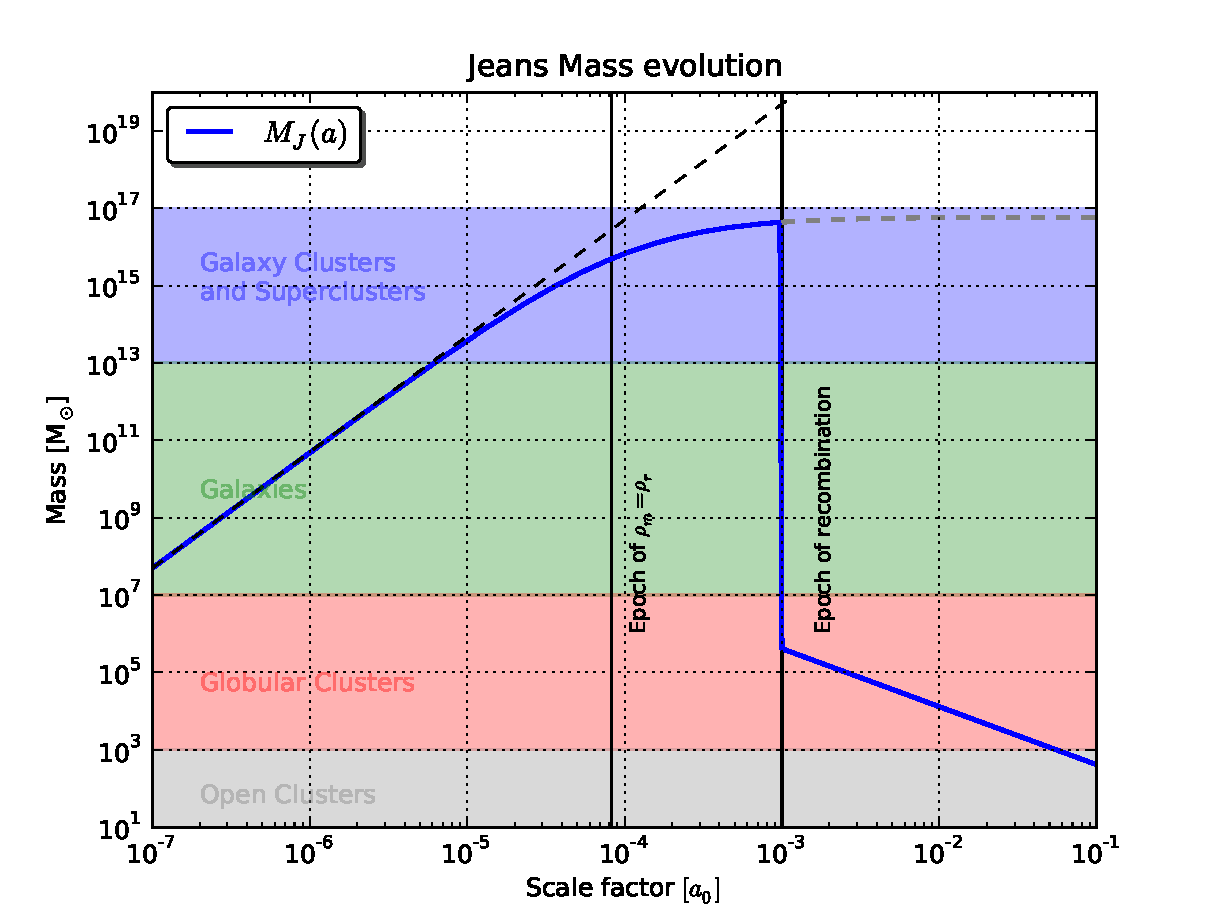
\includegraphics[width=0.9\textwidth]
	{./figures/2_theoretical_framework/Jeans_Mass_Evolution.pdf}

	\caption{\small{Evolución de la masa de Jeans para diferentes estadios
	del universo. En las regiones coloreadas se ilustra el rango típico de 
	masa para varios tipos de estructuras, desde cúmulos estelares abiertos
	hasta cúmulos y supercúmulos de galaxias.}}
	
	\label{fig:JeansMass}
\end{figure}
%.........................................................................	
	

Con el anterior análisis se ha establecido la masa mínima necesaria para 
el colapso de una perturbación, a continuación se estudia la evolución de
tales perturbaciones en medios en expansión. Para esto se hace uso de los
modelos de universo derivados en la subsección 
\ref{subsec:SimpleSolutionsOfTheUniverse} y la ecuación general de evolución
de perturbaciones \ref{eq:ContinuityEquationCMode}.


%.........................................................................
%Solutions to Perturbations Evolution
\begin{itemize}
\item \textbf{Universo Einstein - de Sitter}


Recordando que para este tipo de universo $\Omega_m = \Omega_0 = 1$, usando
la función de Hubble \ref{eq:EinsteindeSitter}, la solución para el factor 
de escala \ref{eq:EinsteindeSitterSolution} y la velocidad del sonido 
derivada de \ref{eq:SoundVelocity} y la ecuación de estado de gas ideal se 
llega a la siguiente expresión para la evolución de las perturbaciones


%.........................................................................	
%Einsten-de Sitter Perturbations
\eq{eq:EinstendeSitterPerturbations}
{ \delta_{\bds k}(a) = \delta_{\bds k, 0} \pr{\frac{a}{a_{\submath{ref}}}}^{1} }
%.........................................................................
donde $\delta_{\bds k, 0}$ son las condiciones del campo en el tiempo de 
referencia $t_{\submath{ref}}$. Otra solución posible es de la forma
$\delta_{\bds k}\propto a^{-3/2}$, pero debido a que es una solución que
decae en el tiempo, no es de interés.


%Radiation Dominated Universe
\item \textbf{Universo dominado por radiación}


Para el caso de perturbaciones en un universo dominado por radiación con
$\Omega_r = \Omega_0 = 1$, usando \ref{eq:RadiationUniverseSolution} se 
llega a


%.........................................................................	
%Radiation Perturbations
\eq{eq:RadiationPerturbations}
{ \delta_{\bds k}(a) = \delta_{\bds k, 0} \pr{\frac{a}{a_{\submath{ref}}}}^{1.22} }
%.........................................................................
donde de nuevo $\delta_{\bds k, 0}$ representa los modos iniciales del 
campo y se ignoran soluciones divergentes.


%Vacuum Dominated Universe
\item \textbf{Universo dominado por vacío}
			

Para un universo de constante cosmológica $\Omega_\Lambda$
\footnote{$\Omega_\Lambda < 1 $ para garantizar convergencia de las soluciones
de la ecuación de Friedmann (ver subsección 
\ref{subsec:SimpleSolutionsOfTheUniverse}).}
se tiene el siguiente comportamiento para la evolución de los modos


%.........................................................................	
%Vacuum Perturbations
\eq{eq:VacuumPerturbations}
{ \delta_{\bds k}(a) = \delta_{\bds k, 0} \pr{\frac{a}{a_{\submath{ref}}}}^{0.58} }
%.........................................................................
\end{itemize}
%.........................................................................


Graficando cada una de estas soluciones se obtiene la figura 
\ref{fig:DeltaEvolution}. Por simplicidad y para ilustrar mejor el 
comportamiento con el factor de escala se normaliza cada solución respecto 
a su valor en el tiempo de referencia $\delta_{\bds k, 0}$. 


Las condiciones iniciales dependen del número de onda comóvil $\bds k$ y
deben ser determinadas a partir de las propiedades estadísticas del campo 
de densidad (ver subsección \ref{subsec:StatisticalProperties}) y de 
medidas observacionales (por ejemplo la radiación cósmica de fondo).

\newpage

%.........................................................................
%Perturbations Evolution
\begin{figure}[htbp]
	\centering
	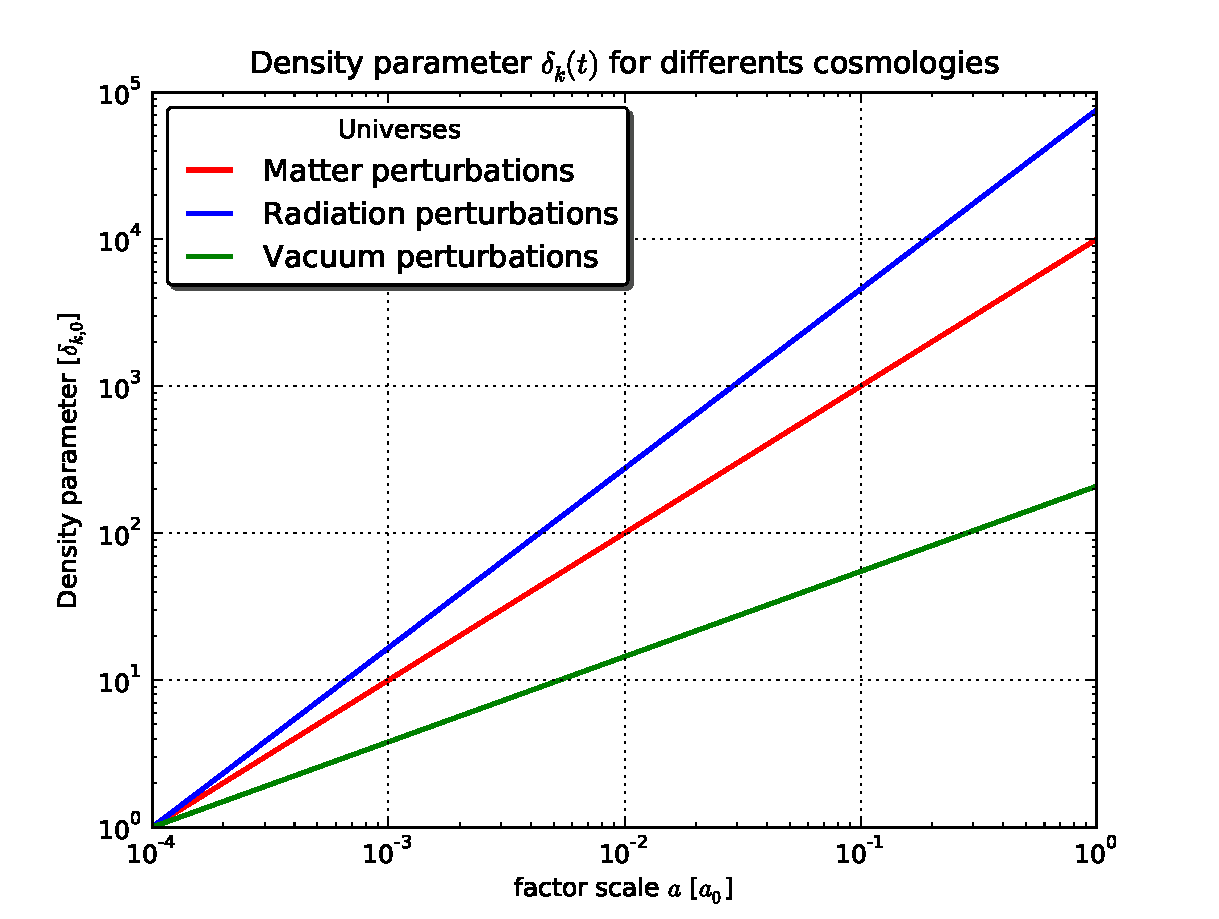
\includegraphics[width=0.9\textwidth]
	{./figures/2_theoretical_framework/Perturbations_Evolution.pdf}

	\caption{\small{Evolución de los modos normales del campo de densidad.
	Por motivos ilustrativos se ha normalizado respecto a las condiciones 
	iniciales.}}
	
	\label{fig:DeltaEvolution}
\end{figure}
%.........................................................................	


	%---------------------------------------------------------------------
	%Statistical Properties and Transfer function
	\subsection{Propiedades Estadísticas y Función de Transferencia}
	\label{subsec:StatisticalProperties}
	%---------------------------------------------------------------------


Una vez determinada la evolución de los modos de densidad es necesario 
compararlos con el universo real. Debido a la naturaleza continua de 
los campos es inviable tratar de determinar de forma ob\-servacional la 
distribución de densidad, más aún, teniendo en cuenta que la mayor parte de 
la materia es oscura, la cual solo puede ser inferida de forma indirecta,
resulta también técnicamente imposible con los instrumentos actuales llevar 
a cabo esta empresa.


A pesar de lo anterior es posible aún medir las propiedades estadísticas
de la distribución de densidad del universo y comparar con lo obtenido de
forma teórica. Para esto se introduce el concepto de funcional de 
probabilidad para un campo continuo $P\cor{ \delta(\bds r,t) }$, definido 
como la probabilidad de que un cierto campo físico tenga la forma funcional 
específica $\delta(\bds r,t)$.


Una manera más conveniente, en términos computacionales, de aplicar el 
formalismo de funcional de probabilidad se logra discretizando el espacio 
en celdas de volumen $\Delta^3 \bds r_i$, de tal forma que una cierta 
forma funcional del campo de densidad $\delta(\bds r,t)$ sea equivalente a 
tener simultáneamente en cada celda $\bds r_i$ del grid el valor 
$\delta_i = \delta(\bds r_i)$, así el funcional de probabilidad se 
transforma en una función de probabilidad conjunta


%.........................................................................
%Probability Functional
\eq{eq:ProbabilityFunctional}
{ P\cor{ \delta(\bds r,t)} \ \ \longrightarrow \ \ 
\mathcal{P}_{\bds{r}}(\delta_1,\delta_2,\cdots,\delta_N;t)  }
%.........................................................................


Teniendo en cuenta la descomposición de Fourier del campo de densidad 
$\delta(\bds r,t)$ en las ecuaciones \ref{eq:FourierFields}, es posible 
definir una función de probabilidad conjunta en el espacio recíproco 
$\mathcal{P}_{\bds k}(\delta_{\bds k_1},\delta_{\bds k_2}, \cdots,
\delta_{\bds k_N};t)$ que caracteriza completamente la probabilidad de 
una distribución específica $\delta_{\bds k}(t)$.


La principal motivación de trabajar en el espacio recíproco de debe a que
es posible usar la aproximación de modos incorrelacionados en la cual se
asume que cada modo evoluciona de forma independiente. En el espacio real 
no es posible realizar esto debido a que el largo alcance de la interacción
gravitacional acopla fuertemente el campo densidad entre diferentes 
lugares. Una consecuencia directa de la anterior aproximación es expresar 
la función de probabilidad conjunta como el producto de $N$ distribuciones
individuales \cite{padmanabhan1995}


%.........................................................................
%Probability Functional Recipro
\eq{eq:ProbabilityJointFour}
{ \mathcal{P}_{\bds k}(\delta_{\bds k_1},\delta_{\bds k_2},
\cdots,\delta_{\bds k_N};t) = \prod_{\bds k_i}g_{\bds k_i}( \delta_{\bds k_i};t )  }
%.........................................................................
donde 


%.........................................................................
%Inverse Fourier Delta
\eq{eq:InverseFourierDelta}
{ \delta_{\bds k} = 
\int_V \delta(\bds r) e^{-i \bds k \cdot \bds r} d^3 \bds r  }
%.........................................................................
$g_{\bds k_i}$ la distribución individual de cada modo, $V=L^3$ el volumen 
de normalización y $\bds k = (2\pi/L)\bds n$, con $\bds n$ un vector de 
componentes enteras que caracterizan el modo específico.


Asumiendo que las perturbaciones primordiales del campo de densidad se 
ori\-ginaron por el proceso de inflación cósmica, es posible demostrar que 
la distribución de los modos normales $g_{\bds k_i}$ es una función 
Gaussiana \cite{padmanabhan1995}. Por conveniencia se descompone en 
coordenadas polares complejas el modo de densidad $\delta_{\bds k} = 
r_{\bds k}\exp\pr{ i \phi_{\bds k} }$, obteniendo la siguiente distribución


%.........................................................................
%Gaussian Distribution
\eq{eq:GaussianDistribution}
{ g_{\bds k}( r_{\bds k}, \phi_{\bds k}; t ) = 
\frac{2(r_{\bds k} dr_{\bds k})}{\sigma_k^2}\pr{ \frac{d\phi_{\bds k}}{2\pi} }
\exp\pr{ -\frac{r_{\bds k}^2}{\sigma_k^2} };\ \ \ \ \ \sigma_k^2 = 2\mu_k^2  }
%.........................................................................
donde $\mu_k^2$ es la varianza de la distribución y $\sigma_k^2$ se 
denomina espectro de potencia. Debido a la asunción de isotropía y 
homogeneidad para el universo de fondo, ambas cantidades solo dependen de 
la magnitud del vector de onda $|\bds k| = k$. También es directo mostrar 
las siguientes propiedades de la distribución del campo


%.........................................................................
%Distribution Properties
\eq{eq:Distribution Properties}
{ \bra \delta_{\bds k} \ket = 0;\ \ \ \ \ 
  \bra |\delta_{\bds k}|^2 \ket = \sigma_k^2;\ \ \ \ \ 
  \bra \delta_{\bds k} \delta_{\bds p}\ket = 0\ \ \ \mbox{si}\ \ \ \
  \bds k \neq \bds p }
%.........................................................................


%.........................................................................
%Initial density
\begin{figure}[htbp]
	\centering
	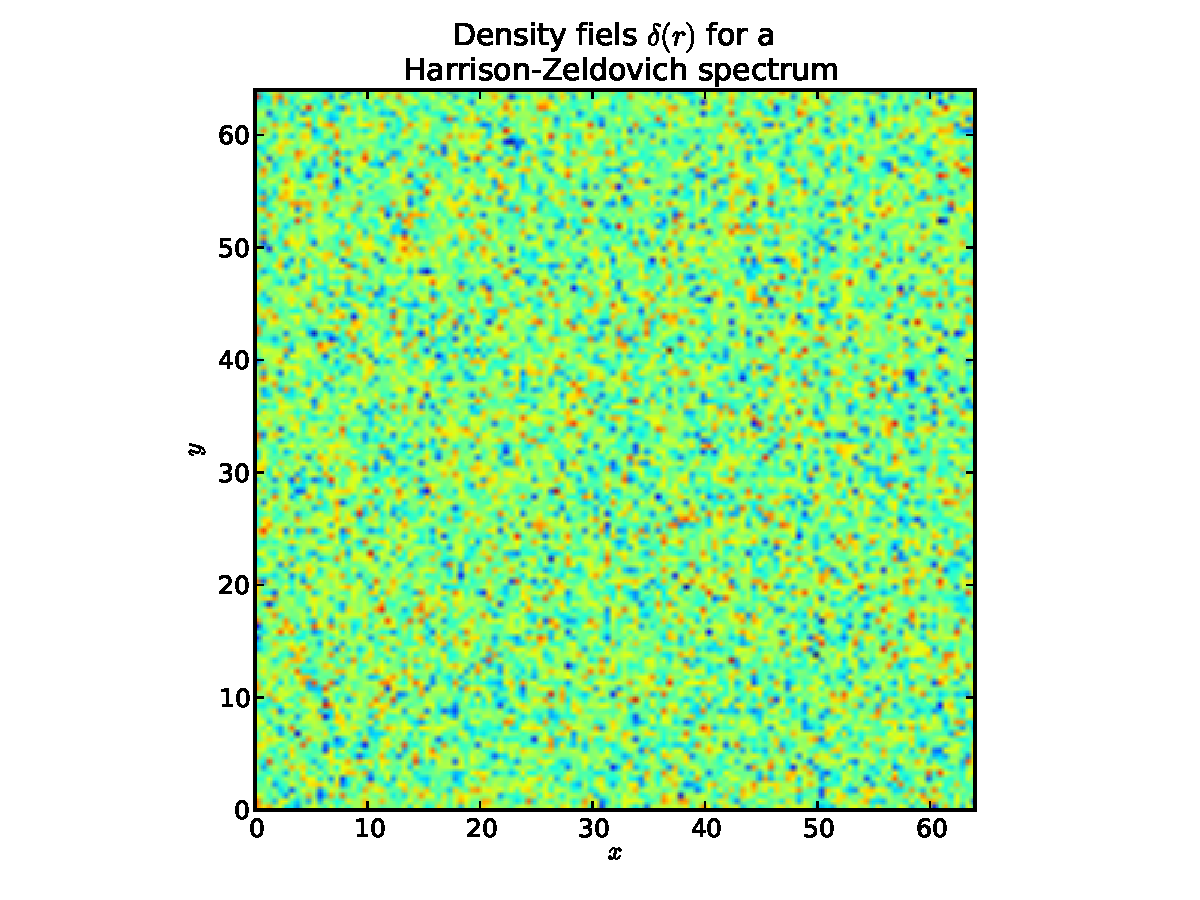
\includegraphics[width=0.9\textwidth]
	{./figures/2_theoretical_framework/Initial_Density.pdf}

	\caption{\small{Distribución inicial de perturbaciones para el campo
	de contraste de densidad a partir de la distribución Gaussiana 
	\ref{eq:GaussianDistribution} y el espectro de potencia de Harrison-
	Zeldovich $\sigma_k \propto k$.}}
	
	\label{fig:InitialDensity}
\end{figure}
%.........................................................................	


Una cantidad que puede ser evaluada directamente es la función de 
correlación de dos puntos $\xi(\bds r) \equiv \bra \delta(\bds r' + \bds r)
\delta(\bds r') \ket$, definida como la probabilidad de tener una 
perturbación a una distancia $\bds r$ de otra. Es una medida directa del 
grado de anisotropía y las propiedades de clustering de una distribución.


%.........................................................................
%Two Points Correlation Function
\begin{eqnarray}
\nonumber
\xi(\bds r) = \bra \delta(\bds r' + \bds r) \delta(\bds r') \ket &=& 
\frac{1}{V^2}\sum_{\bds k, \bds p} \bra \delta_{\bds k} \delta_{\bds p}^*\ket
\exp\cor{ i\bds k \cdot(\bds r' + \bds r)- i\bds p \cdot \bds r' } \\
\label{eq:2PCorrelation}
&=& \int \frac{V^{-1}}{(2\pi)^3}\sigma_k^2 e^{i \bds k \cdot \bds r} d^3 \bds k
\end{eqnarray}
%.........................................................................
donde en la última línea se ha realizado el límite al continuo. La 
expresión \ref{eq:2PCorrelation} muestra que $\sigma_k^2$ es la 
transformada de Fourier de la función de correlación, es decir


%.........................................................................
%Two Points Correlation Function Fourier
\eq{eq:2PCorrelationF}
{ V^{-1}\sigma_k^2 = \int \xi(\bds r) e^{-i\bds k\cdot \bds r}d^3 \bds r }
%.........................................................................


La anterior relación junto con la distribución Gaussiana del campo muestra 
que tanto el espectro de potencia como la función de correlación contienen
toda la información estadística del campo de densidad en el régimen lineal.
En caso de asumir una distribución no-Gaussiana es necesario tener más
momentos de la distribución, tal como la función de correlación de tres 
puntos, etc.


			%-------------------------------------------------------------
			%Harrison-Zeldovich Power Spectrum
			\subsubsection*{Espectro de potencia de Harrison-Zeldovich}
			%-------------------------------------------------------------
			

Una primera aproximación al espectro de potencia, y que puede ser 
demostrada con el modelo de inflación cósmica para las perturbaciones 
primigenias \cite{padmanabhan1995}, es una ley de potencia de la forma


%.........................................................................
%Power Spectrum power
\eq{eq:PowerSpectrumPower}
{ \sigma_k^2 = A k^{n_s} }
%.........................................................................
donde $A$ es un factor de normalización y $n$ es el índice espectral. En 
el caso específico en que $n_s=1$ se denomina espectro de potencia de 
Harrison-Zeldovich y es invariante de escala \footnote{El valor determinado 
observacionalmente es muy cercano $n_s = 0.963$ (ver tabla
\ref{tab:CosmologicalParameters}).}.


Para determinar el factor de normalización es común aplicar un filtro a 
los modos normales que contribuyen al campo de densidad, con esto la 
función de correlación queda


%.........................................................................
%Two Points Correlation Function Fourier with Filter
\eq{eq:Filter2PCorrelation}
{ \xi(\bds r;R) = \int \frac{V^{-1}}{(2\pi)^3}\sigma_k^2 
e^{i \bds k \cdot \bds r} \tilde{W}(k;R) d^3\bds k }
%.........................................................................
donde $R$ determina la escala máxima a partir de la cual se aplica el 
filtro en los modos del campo y $\tilde{W}(k;R)$ es la transformada de
Fourier de la función de filtro. En especial se define la dispersión en el
espacio real asociada a una escala $R$ como $\sigma^2_R = \bra \delta^2 \ket=
\xi(0; R)$, este parámetro puede ser determinado observacionalmente a partir
de surveys de galaxias y de la radiación cósmica de fondo, en especial el 
valor estándar definido por el WMAP7 es $\sigma^2_8 = \xi(0; R = 
8 \mbox{ Mpc}/h) = 0.801$ (ver tabla \ref{tab:CosmologicalParameters}), con
esto se llega a


%.........................................................................
%Normalization Expression
\eq{eq:Normalization}
{ \sigma_8^2 = A\int \frac{V^{-1}}{(2\pi)^3} k^{n_s}
 \tilde{W}(k;R=8 \mbox{ Mpc}/h) d^3\bds k }
%.........................................................................
de esta forma, a partir de los valores medidos de $n_s$ y $\sigma_8^2$, es
posible encontrar la normalización del espectro de potencia.


			%-------------------------------------------------------------
			%Transfer Function
			\subsubsection*{Función de Transferencia}
			%-------------------------------------------------------------
			

Finalmente para el régimen lineal se introduce el concepto de función de 
trans\-ferencia $T_{\bds k}(t)$, definida a partir de la siguiente 
expresión


%.........................................................................
%Transfer function Definition
\eq{eq:TransferFunction}
{ \delta_{\bds k}(t) = T_{\bds k}(t) \delta_{\bds k}(t_i) }
%.........................................................................
donde $t_i$ es un tiempo de referencia, normalmente la época de 
recombinación en el caso de perturbaciones de materia.


De la expresión \ref{eq:TransferFunction} se infiere que la función de 
transferencia contiene toda la información dinámica de las perturbaciones,
más aún, de la definición \ref{eq:Distribution Properties} para el espectro
de potencia se tiene


%.........................................................................
%Power Spectrum and Transfer Function
\eq{eq:PkTransferFunction}
{ \sigma_k(t) = \sigma_k(t_i)|T_k(t)|^2 = Ak^{n_s} |T_k(t)|^2 }
%.........................................................................
donde se ha asumido un espectro de potencia de Harrison-Zeldovich para el 
tiempo de referencia. Con esto finalmente se concluye que la función de 
transferencia también permite obtener todas las propiedades estadísticas 
del campo durante el tiempo en que el régimen lineal es válido.


El cálculo de la función de transferencia es generalmente complejo y 
requiere realizarse numéricamente \footnote{\texttt{CMBFAST} es un 
software bastante conocido para este propósito 
\url{http://lambda.gsfc.nasa.gov/toolbox/tb_cmbfast_ov.cfm}}, además
depende de las propiedades específicas de la especie asociada a la
perturbación. Como un ejemplo, en el caso de perturbaciones de materia 
oscura debe ser especificado el tipo de partículas que la componen, ya 
sean partículas livianas relativistas (materia oscura caliente) o 
partículas pesadas no relativistas (materia oscura fría). Entre ambos 
casos la función de transferencia y el espectro procesado 
\ref{eq:PkTransferFunction} difieren bastante debido a las diferentes 
ecuaciones de estado asociadas a cada tipo.


En el caso de perturbaciones adiabáticas (isoentrópicas) de materia 
oscura fría puede usarse la siguiente aproximación analítica para la 
época actual \cite{longair2008}


%.........................................................................
%Transfer Function CDM
\eq{eq:TransferFunctionCDM}
{ T_k \approx \frac{ \ln\pr{ 1 + 2.34 q } }{2.34 q}
\cor{ 1 + 3.89 q + \pr{ 1.61 q }^2 + \pr{ 5.46 q }^3 + \pr{ 6.71 q }^4}^{-1/4} }
%.........................................................................
donde $q \equiv k/\Omega_0 h^{2} \mbox{ Mpc}^{-1} $.


En la siguiente figura se ilustra la función de transferencia 
\ref{eq:TransferFunctionCDM} junto con el espectro de potencia procesado

%.........................................................................
%Transfer Function CDM
\begin{figure}[htbp]
	\centering
	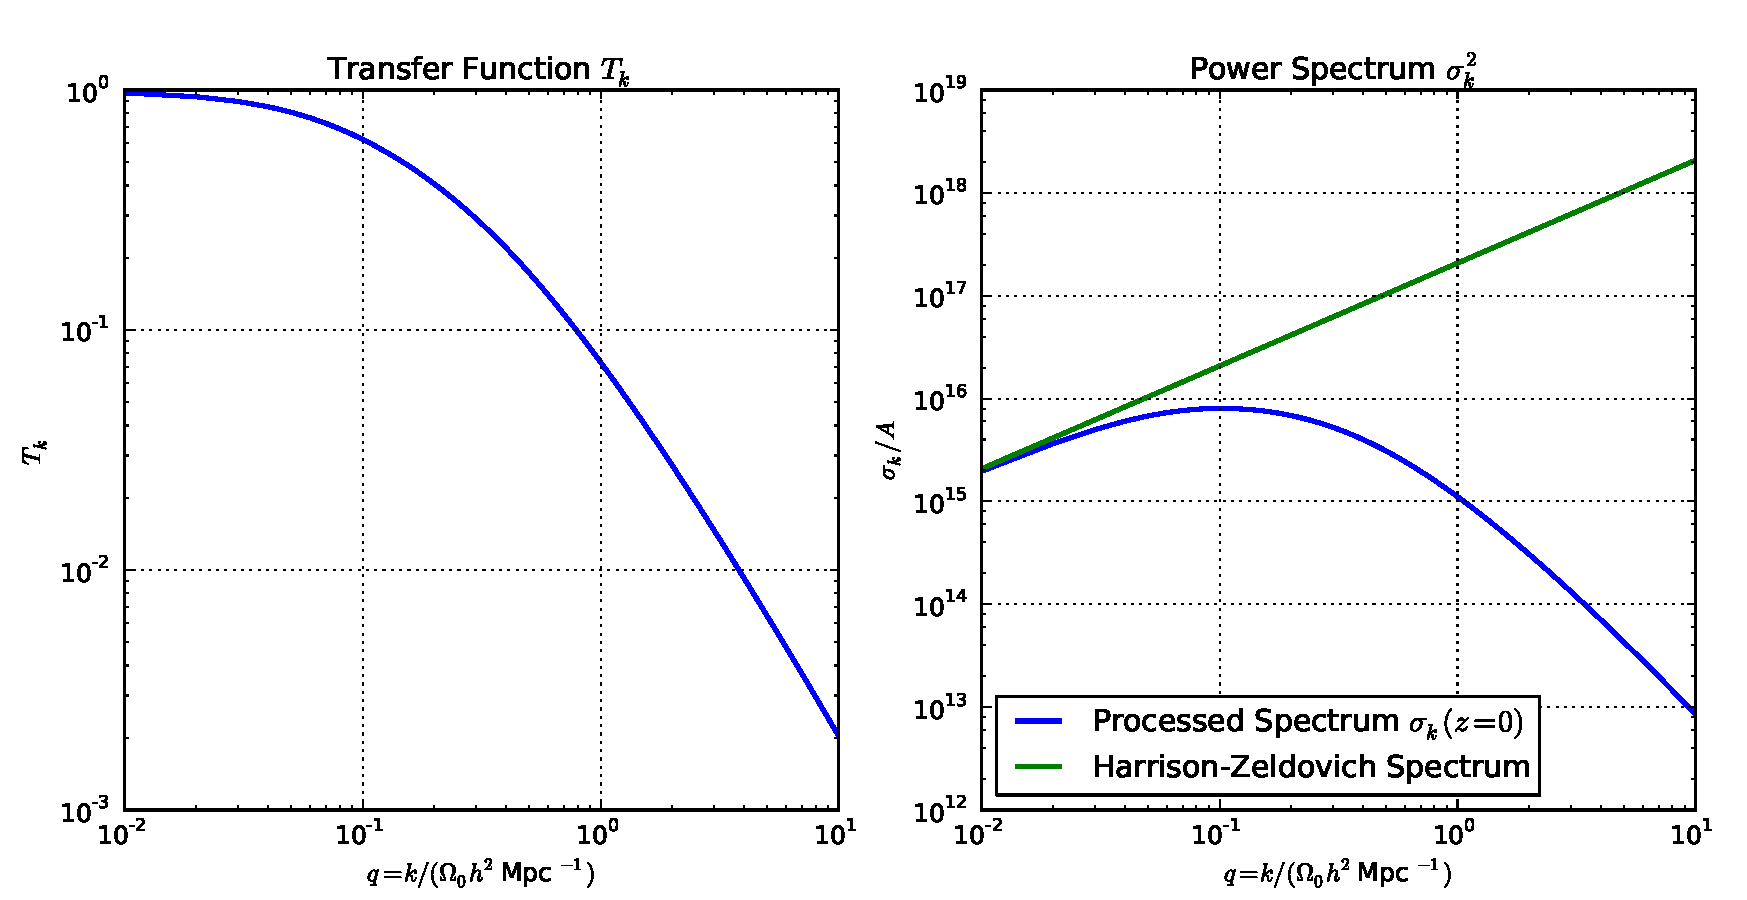
\includegraphics[width=0.9\textwidth]
	{./figures/2_theoretical_framework/Transfer_Function.pdf}

	\caption{\small{Función de transferencia para materia oscura fría en la
	época actual \cite{longair2008} (Izquierda). Comparación entre el 
	espectro de potencia inicial, Harrison-Zeldovich, y el espectro de 
	potencia procesado (derecha).}}
	
	\label{fig:TransferFunctionCDM}
\end{figure}
%.........................................................................	


De todo el formalismo desarrollado en esta sección se concluye que el 
objetivo final para la caracterización del régimen lineal es obtener la 
función de transferencia, ya que esta determina completamente la 
evolución del universo en épocas tempranas donde hay alta homogeneidad e
isotropía en todas las escalas.


%*************************************************************************




%*************************************************************************
%NonLinear Structure Formation
\section{Régimen No Lineal de Formación de Estructuras}
\label{sec:NonLinearStructureFormation}


En el régimen lineal se describe el proceso de formación de estructuras 
como perturbaciones en un universo de fondo homogéneo e isotrópico. Cuando
las perturbaciones crecen tal que $\delta \gtrsim 1$ la autogravedad de 
los modos acopla fuertemente el campo de forma local y e invalida la 
aproximación lineal. Los procesos físicos asociados al régimen no lineal
son altamente complejos e inclusive algunos no son bien entendidos en la 
actualidad, esto hace que solo sea posible abordar satisfactoriamente el 
problema a través de simulaciones numéricas (ver capítulo 
\ref{cha:N-BodySimulations}).


%.........................................................................
%Nonlinear Universe
\begin{figure}[htbp]
	\centering
	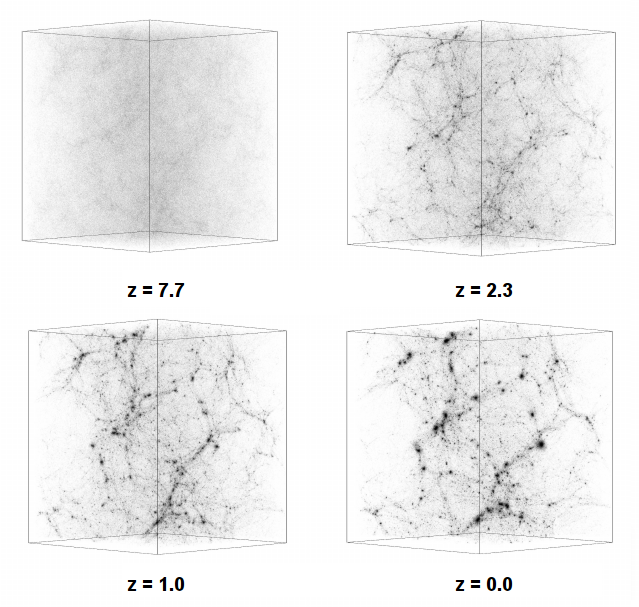
\includegraphics[width=0.9\textwidth]
	{./figures/2_theoretical_framework/Nonlinear.png}

	\caption{\small{Evolución de una simulación numérica de materia oscura
	en una caja de 40 Mpc$/h$, iniciando en un estado de alta homogeneidad 
	(arriba-izquierda) hasta la época actual de estructuras altamente no 
	lineales (abajo-derecha). Tomado de 
	\url{http://www.astro.utu.fi/research/CosmoS/lss/lss_p1.shtml}}}
	
	\label{fig:NonLinearUniverse}
\end{figure}
%.........................................................................


La figura \ref{fig:NonLinearUniverse} corresponde a una simulación 
numérica de materia oscura para el universo en régimen no lineal. En esta 
pueden ser apreciadas algunas propiedades emergentes tales como la 
anisotropía e inhomogeneidad a escalas peque\-ñas ($\sim$ Mpc), la 
formación y clustering de estructuras altamente no lineales y la aparición 
de un patrón de red a grandes escalas (red cósmica).


	%---------------------------------------------------------------------
	%Zeldovich's Approximation
	\subsection{Aproximación de Zeldovich}
	\label{subsec:Zeldovich'sApproximation}
	%---------------------------------------------------------------------
	

A pesar de la complejidad del régimen no lineal, cuando las perturbaciones 
en el campo de densidad aún no son mucho mayores que el valor de fondo 
puede realizarse una desarrollo analítico de la evolución, esto es conocido
como aproxi\-mación de Zeldovich y fue desarrollada en 1970 por Yakov 
Zeldovich en \cite{zeldovich1970}. Para formular esta aproximación es 
conveniente expresar de nuevo el campo de contraste de densidad 
$\delta(\bds r)$ en términos de coordenadas comóviles y no respecto a los 
modos normales de Fourier, esto debido a que en este régimen los modos no 
son independientes y usarlos no simplifica el tratamiento, a diferencia 
del régimen lineal. 


Usando el marco de referencia Lagrangiano de una cierta porción de fluido
o distribución de materia, su trayectoria $\bds r_f$ puede ser descrita 
mediante la siguiente expresión


%.........................................................................
\eq{eq:ZeldovichTrayectory}
{ \bds r_f( t,\bds q ) = a(t)\bds r = a(t)\cor{ \bds q + \bds \Psi(\bds q,t) } }
%.........................................................................
donde $\bds r$ es la posición comóvil de la porción de fluido, $\bds q$ 
su coordenada Lagrangiana inicial cuando el fluido no está perturbado y 
$\bds \Psi(\bds q,t)$ se denomina función de desplazamiento y da cuenta de 
las perturbaciones en el medio. 


A partir de la ecuación de evolución del campo de contraste de densidad 
\ref{eq:DeltaEvolution} es posible demostrar que el campo de desplazamiento 
$\bds \Psi(\bds q,t)$ satisface \cite{Yoshisato2006}


%.........................................................................
%Displacement Differential Equation
\eq{eq:Displacement}
{ \der{^2  \bds \Psi}{t^2} + 2H\der{\bds \Psi}{t} =
 \frac{ 3}{2}H^2 \bds \Psi  }
%.........................................................................
de esto se obtiene finalmente


%.........................................................................
%Displacement Explicit Form
\eq{eq:DisplacementForm}
{ \bds \Psi = \frac{3}{2}H_0^{-2}a(t)\nabla \Phi  }
%.........................................................................
donde $\Phi$ es el potencial gravitacional efectivo asociado al campo de 
densidad por medio de la ecuación de Poisson \ref{eq:PoissonEquationC}.


Expresando la conservación de la masa en términos de las coordenadas 
comóviles y las coordenadas Lagrangianas iniciales, se debe satisfacer


%.........................................................................
%Mass Conservation
\eq{eq:MassConservation}
{ \rho(\bds r, t)d^3 \bds r = \bar{\rho}(t)d^3 \bds q  }
%.........................................................................
calculando ahora el Jacobiano $\partial q_i / \partial r_j$ de la 
transformación $\bds r \rightarrow \bds q$, el campo de densidad perturbado 
pude se escrito como \cite{padmanabhan1995}


%.........................................................................
%Perturbed Field Density
\eq{eq:PerturbedFieldDensity}
{ \rho(\bds r, t) = \frac{\bar \rho (t)}{\pr{ 1 - a(t) \lambda_1(\bds q)}
\pr{ 1 - a(t) \lambda_2(\bds q)}\pr{ 1 - a(t) \lambda_3(\bds q)} } }
%.........................................................................
donde $-\lambda_i(\bds q)$ son los autovalores del Jacobiano y están 
ordenados de tal forma que $\lambda_1\geq\lambda_2\geq\lambda_3$. Cada uno
de estos autovalores pueden ser interpretados de forma geométrica como un 
indicador del colapso o expansión de una porción de fluido en la dirección
correspondiente al autovector respectivo, así por ejemplo si $\lambda_i > 0$,
implica que el campo de densidad está colapsando localmente en la dirección 
del autovector $\bds u_i$, mientras que $\lambda_i < 0$ implica una 
expansión en la misma dirección.

\
%.........................................................................
%Zeldovich Approximation Comparison
\begin{figure}[htbp]
	\centering
	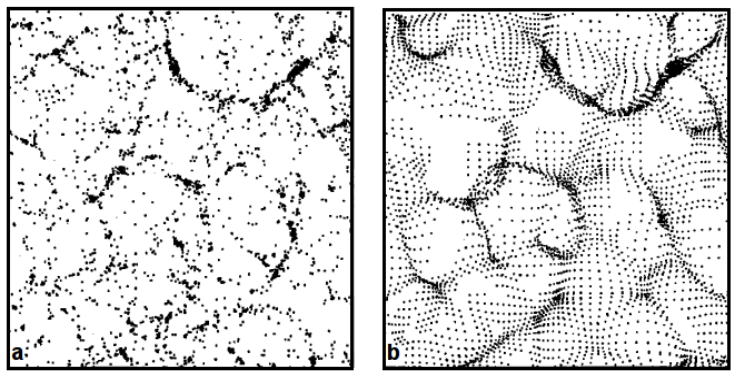
\includegraphics[width=0.9\textwidth]
	{./figures/2_theoretical_framework/Zeldovich_Approximation.png}

	\caption{\small{Comparación de la evolución en régimen no lineal entre
	una simulación de N-cuerpos (a), y la aproximación de Zeldovich (b).
	En ambos casos se usan las mismas condiciones iniciales. Tomado de 
	\cite{longair2008}. }}
	
	\label{fig:ZeldovichComparison}
\end{figure}
%.........................................................................


Finalmente en la figura \ref{fig:ZeldovichComparison} se muestra una 
comparación entre una simulación numérica de N-cuerpos y la aproximación 
de Zeldovich, puede notarse una alta semejanza visual en las estructuras 
obtenidas en los dos casos al final de la evolución, demostrando la alta 
precisión del método. En la sección \ref{sec:EnvironmentCharacterization}
se hace uso de la idea general planteada en la aproximación de Zeldovich 
respecto a los autovalores del Jacobiano de la transformación, para la 
construcción de esquemas de clasificación del entorno cosmológico a partir 
de los autovalores de otras cantidades físicas más adecuadas para la 
descripción de la dinámica local del campo de densidad, tales como el 
tensor de marea o el tensor de velocidad peculiar.


%*************************************************************************